\documentclass[11pt]{article}
% \def\StudentVersion{}
\usepackage{../common}
\title{Constraint Satisfaction}
\date{}

\def\LecStr{Alexander Rush}
\def\LecNum{3}
\def\LecTitle{Lecture Notes on Constraint Satisfaction}
\def\LecDate{}

\begin{document}
\MakeScribeTop{}

\tableofcontents
\section{Introduction}

In the first set of lectures we have looked at two types of models, generic search models
and models for game playing. Both utilize a state representation that evolves through the
result of actions. In this section we consider a different model formulation, known as a constraint
satisfaction problem (CSP). This model will use a more restrictive representation that will require
us to specify specific constraints about the world. Instead of actions, CSPs
require us to specify a  fixed set of variables and constraints. The goal will be to find an assignment to
the variables that satisfies all of the constraints.

After defining CSPs we will look at algorithms for solving them. We will
see that CSPs can be solved using similar search algorithms as we saw
in the previous classes. However the main benefit of this model is it
allows us to employ general search algorithms without having to define
problem specific heuristics. In addition CSPs also give us a framework
for utilizing \textbf{local search}, a different style of algorithm
that can be a very effective means for solving constrained
problems.

\section{A Running Example: Map Coloring}


For these lectures, we will use the running example of map
coloring. In particular we will attempt to find a 4-coloring of a map
shown below. That this is always possible is the conclusion of famous
mathematical theorem first proven 1976 (with the assistance of
algorithmic techniques). While we will not go into details of the
proof, coloring a specific map fits nicely as an example of the CSP
framework. The theorem states that given a map and four distinct colors it is
possible to return a coloring such that no two adjacent contiguous
areas are assigned the same color.

We will apply this approach to a map of the Cambridge area
shown below. For this problem we will define the coloring set as $\msc{Colors} =
\{\mathrm{R, Y, O, B}\}$, i.e. red, yellow, orange, and blue. Specify
a valid coloring relationship using set notation: 

\[\msc{DifColor} = \{c_1, c_2 \in \msc{Color} : c_1 \neq c_2 \}\].

\begin{figure}[h]
  \centering
  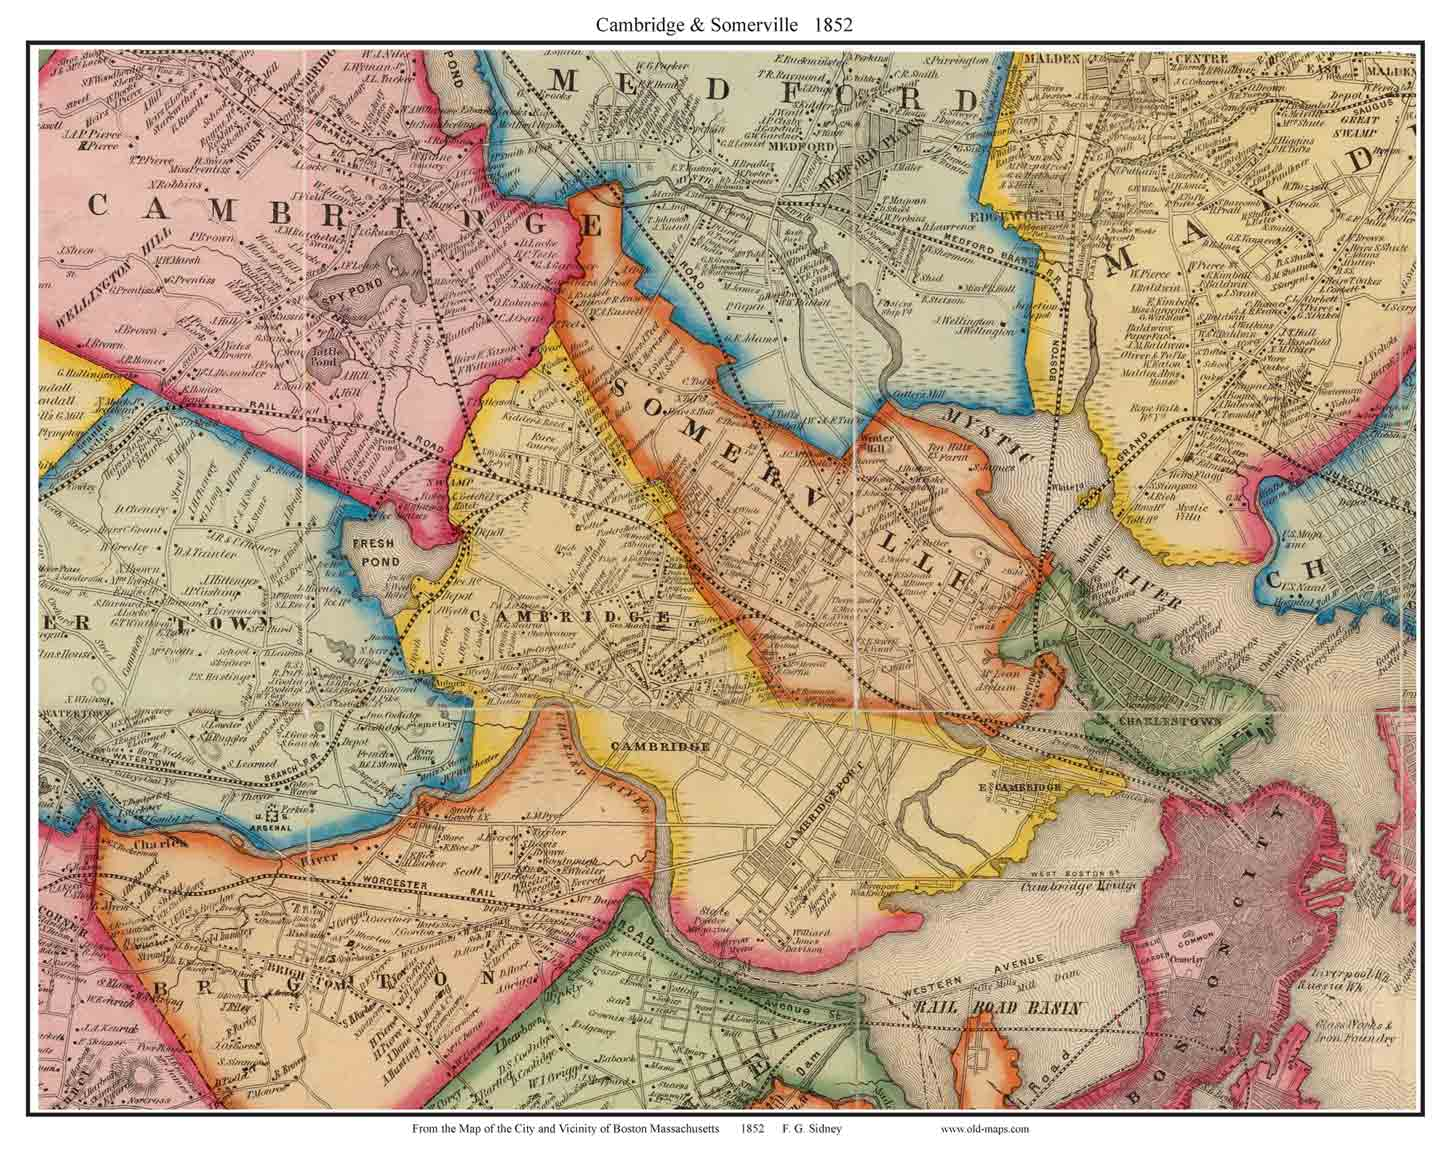
\includegraphics[width=0.8\linewidth]{pics/CambridgeSomerville_1852_web}
  \label{fig:camb}
  \caption{Cambridge-area circa 1852. Best viewed in color.}
\end{figure}



\section{Constraint Satisfaction Problems}

\subsection{Formulation}

We begin by giving a formal model of a constraint satisfaction problem. Note that our definition differs slightly from that given in AIMA in that we try to give a more specific definition of constraints.


A constraint satisfaction problem (CSP) defines a sets of \textbf{variables} which are jointly constrained. Formally a constraint satisfaction problem is defined by the following elements:

 \air
\begin{center}
\begin{tabularx}{\linewidth}{llX}
  \toprule
  Name (AIMA) & Type & Description \\
  \midrule
\\
 Variables & $X_1, \ldots, X_n$ &  Name of each variable in the problem.\\\\
 Labels/ Variable Domains & $\mcD_1, \ldots, \mcD_n$&   The set of labels that each variable can take on, e.g. domain $\mcD_i$  corresponds to $X_i$ for all $i \in \{1, \ldots, n\} $\\\\
 \midrule\\
 Factors & $F_1, \ldots,F_m$ & Each factor is a list of variables, constrained by that factor, for example $F_2 = ( X_1, X_4, X_{10})$  \\\\
 Constraints/Factor Domains &  $\mcR_1, \ldots, \mcR_m$ & The set of labels each variable constrained by a factor can simultaneously take on. $\mcR_i$ corresponds to factor $F_i$ for all $i \in \{1, \ldots, m\} $.     \\\\
 \bottomrule
\end{tabularx}
\end{center}


As an example, say we have three variables $X_1, X_2, X_3$ all with
the same domains $\mcD_1 = \mcD_2 = \mcD_3 = \{\mathrm{A, B, C}\}$. We
could then have a factor $F_1 = (X_1, X_3)$ with constraint $\mcR_1 =
\{(\mathrm{A, B}), \mathrm{(A, C})\} \rangle $. This says that the
only two valid labels for $X_1$ and $X_3$ are $X_1 = A, X_3 = B$ and
$X_1 = A, X_3=C$. It says nothing about $X_2$.  While a single factor
can constrain many variables, we will mainly consider
pairwise factors, also known as \textbf{arcs}.

Instead of paths as in search, we will be interested in assignments for CSP. In particular:  

\begin{defn}
A \textbf{assignment} $A \in (\mcD_1 \cup \{\epsilon\}) \times \ldots \times (\mcD_n \cup \{\epsilon\})$ consists of a label (or blank) for each variable. We say the assignment is \textbf{partial} if it includes $\epsilon$, and \textbf{complete} if it does not. 
\end{defn}


\begin{defn}
  A partial/complete assignment is \textbf{consistent} if it
  does not violate any constraints. That is for each factor $(X_i, X_j)$,
  the assignment is $(A_i, A_j)$ is in the set of valid relations or
  at least one is $\epsilon$.
\end{defn}

A complete, consistent assignments is analogous to a solution path.
For CSPs, we will treat all consistent paths as equally acceptable,
i.e. there is no costs associated with assignments. (Note, however
there are important variants of the CSP formalism that do model this
idea of an assignment costs.)


\subsection{Factor Graph}

We can represent a constraint satisfaction problem using a graphical
representation known as a \textbf{factor graph} (called a constraint hypergraph
in AIMA).  A factor graph is an undirected graph with two types of
nodes: \textbf{variable nodes}, which are drawn as circles and
\textbf{factor nodes} drawn as squares. There are $n$ variable nodes
in the graph, and $m$ factor nodes. For each factor $F_i = (X_{f_1},
\ldots, X_{f_o})$ we connect the corresponding factor node $F_i$ to
the corresponding variable nodes $X_{f_1}$ through $X_{f_o}$.

Note that the factor graph makes no attempt to represent labels or
constraints at all, it only represents  which variables are 
constrained by which factors.

\subsection{Graph Coloring}


\begin{exercise}
    Let's now define the CSP for this graph coloring problem.
\end{exercise}

 \air
\begin{center}
\begin{tabularx}{\linewidth}{lX}
  \toprule
 Variables & \censor{$X = \langle \mathrm{Cambridge, Somerville, Brighton, Boston, Watertown} \rangle$}   \\\\
 Labels & \censor{$\mcD_1 = \msc{Colors}, \ldots, \mcD_n = \msc{Colors}$}   \\\\
 \midrule \\ 
 Factors & \censor{\begin{eqnarray*}
   F_1 &= & (\mathrm{Cambridge, Somerville}),\\
   F_2 &= &(\mathrm{Cambridge, Boston}), \\  
   F_3 &= &(\mathrm{Cambridge, Watertown}),  \\  
   F_4 &= &(\mathrm{Cambridge, Brighton}), \\ 
   F_5 &= &(\mathrm{Brighton, Boston}), \\  
   F_6 &= & (\mathrm{Brighton, Watertown})  
   \end{eqnarray*}} \\\\
 Constraints &  \censor{$\mcR_1 = \msc{DifColor},  \ldots, \mcR_6 = \msc{DifColor} $}  \\\\
 \bottomrule
\end{tabularx}
\end{center}
\air

So for this problem are $n= 5$ variables and $m=6$ factors, each is also an arc. The representation is much easier to visualize as a factor graph. Below we shows a factor graph representation of the same CSP. 
However note it does not explicitly show the constraints of the graph. 

\air
\begin{figure}[h]
  \centering
  \begin{tikzpicture}
    \draw node(s)[draw, ellipse] at (2.5, 2.5){Somerville};
    \draw node(w)[draw, ellipse] at (-5, 0){Watertown};
    \draw node(c)[draw, ellipse] at (0, 0){Cambridge};
    \draw node(br)[draw, ellipse] at (-2, -2.5){Brighton};
    \draw node(bo)[draw, ellipse] at (2.5, -2.5){Boston};
    \draw (br) -- node[draw, fill]{} (c);
    \draw (br) -- node[draw, fill]{} (w);
    \draw (c) -- node[draw, fill]{} (s);
    \draw (c) -- node[draw, fill]{} (w);
    \draw (br) -- node[draw, fill]{} (c);
    \draw (c) -- node[draw, fill]{} (bo);
    \draw (br) -- node[draw, fill]{} (bo);
    
  \end{tikzpicture}
  \label{fig:cambfactor}
  \caption{Factor graph showing the constraints for the Cambridge 
  graph coloring problem. }
\end{figure}
\air

\begin{exercise}
  Generate: 

  \begin{enumerate}
  \item A complete, consistent assignment for this problem.
  \item An incomplete, consistent assignment for this problem.
  \item An complete, inconsistent assignment for this problem.
  \end{enumerate}
\end{exercise}

\censor{
\begin{enumerate}
\item A complete, consistent assignment is show in Figure~\ref{fig:camb}. In our notation this assignment is represented as $\langle \mathrm{Y, O, O, G, B} \rangle$.
\item   If we had the same graph, but had not yet assigned a color to Cambridge we would write it as $\langle \epsilon, \mathrm{ O, O, G, B} \rangle$. This assignment is incomplete, but consistent.
\item  Alternatively if we flip the color of Cambridge and Somerville we end up with  $\langle \epsilon, \mathrm{O, Y, O, G, B} \rangle$ which is complete but inconsistent.
\end{enumerate}
}

\subsection{Example 2: Part-of-Speech Tagging}

Let's consider a rather different example from the field of natural 
language processing. Imagine we are implementing a system like SIRI
and we are given a crucial question such as ``Where is Toscanini's located?''.
One of the first steps for handling such a question is to label each word 
with its part-of-speech tag. 

We can model this problem using a CSP. The factor graph for this
problem is shown in Figure~\ref{fig:tag}. We have a factor connecting
each of the part-of-speech tags and a factor connecting each word to
its tag.  Here the domain of each tag variable consists of a
part-of-speech tag $\msc{Tags} = \{ \mathrm{Noun, Adjective, Verb,
  ... } \}$, and the word variable domain will consist of single word
$\mcD_1 = \{\mathrm{Where}\}$. The constraints will ensure two things:

\begin{enumerate}
\item Each tag is a match its word $\msc{TagDict}$ 
\item Neighboring tags are consistent $\msc{TagCons}$
\end{enumerate}

The first constraint will ensure that the tag of each word is consistent
with the tags previously seen for that word. Many words in English are consistent 
with several different tags.  The second constraint will ensure that the 
tag sequence is consistent with what is common in English.

If we can find a complete consistent assignment here, it is likely to
give a good tagging of the sentence.


\vspace{1cm}
\ifthenelse{\isundefined{\StudentVersion}}{
\censor{}

  \scalebox{0.8}{
  \begin{tikzpicture}
    \draw node(ta)[draw, ellipse] at (0, 1){Tag1};
    \draw node(tb)[draw, ellipse] at (5, 1){Tag2};
    \draw node(tc)[draw, ellipse] at (10, 1){Tag3};
    \draw node(td)[draw, ellipse] at (15, 1){Tag4};

    \draw node(wa)[draw, ellipse] at (0, -1){Word1 (\textit{Where}) };
    \draw node(wb)[draw, ellipse] at (5, -1){Word2 (\textit{is})};
    \draw node(wc)[draw, ellipse] at (10, -1){Word3 (\textit{Toscanini's})};
    \draw node(wd)[draw, ellipse] at (15, -1){Word4 (\textit{located?})};
    
    \draw (ta) -- node[draw, fill]{} (tb);
    \draw (tb) -- node[draw, fill]{} (tc);
    \draw (tc) -- node[draw, fill]{} (td);
    \draw (ta) -- node[draw, fill]{} (tb);

    \draw (ta) -- node[draw, color=blue,fill]{} (wa);
    \draw (tb) -- node[draw, color=blue,fill]{} (wb);
    \draw (tc) -- node[draw, color=blue,fill]{} (wc);
    \draw (td) -- node[draw, color=blue,fill]{} (wd);

  \end{tikzpicture}
}
}{
\censor{}
\vspace{5cm}

}

\begin{exercise}
  Give some explicit constraints that might be used in this model.  
\end{exercise}


  \begin{itemize}
  \item The word 'is' most always be a verb.
  \item The Adj/Noun
  \end{itemize}




\section{Consistency Checks}

One benefit of the CSP formalism is that it allows us to make 
direct \textbf{inferences} about unassigned variables based on a
current partial assignment of the CSP. This can be done through 
\textbf{consistency} checks that recalibrate the domains of variables
based on neighboring domains. 

Consider for example a consistent partial assignment to the 
map coloring CSP.

\[\langle \epsilon, \epsilon, \mathrm{O, G, B} \rangle\]
\air 

\begin{figure}[h]
  \centering
  \begin{tikzpicture}
    \draw node(s)[draw, ellipse] at (2.5, 2.5){Somerville};
    \draw node(w)[draw, ellipse, fill=blue] at (-5, 0){Watertown};
    \draw node(c)[draw, ellipse] at (0, 0){Cambridge};
    \draw node(br)[draw, ellipse, fill=orange] at (-2, -2.5){Brighton};
    \draw node(bo)[draw, ellipse, fill=green] at (2.5, -2.5){Boston};
    \draw (br) -- node[draw, fill]{} (c);
    \draw (br) -- node[draw, fill]{} (w);
    \draw (c) -- node[draw, fill]{} (s);
    \draw (c) -- node[draw, fill]{} (w);
    \draw (br) -- node[draw, fill]{} (c);
    \draw (c) -- node[draw, fill]{} (bo);
    \draw (br) -- node[draw, fill]{} (bo);
    
  \end{tikzpicture}
  \label{fig:cambcolor}
  \caption{A consistent partial coloring of the Cambridge area. }
\end{figure}

Our consistency check will ask what is the effective domain 
of the unassigned variables: Somerville and Cambridge.
The algorithm will go through each factor and filter the domains of its constrained variables.
 
The algorithm proceeds as follows: 

\begin{enumerate}
\item We start with the Somerville-Cambridge factor and check whether any of 
  it constrains out any of Somerville's assignments. 
  However since the Cambridge variable could at this point be any 
  color, we cannot limit out any of the coloring options for Somerville.
\item Next we check the other factors around Cambridge. In this case it has three factors each
  with assigned neighbors.  Going through the constraints, we see that
  (1) the factor with Watertown means it cannot be blue, (2) the
  factor with Brighton means it cannot be orange, (3) the factor with
  Boston means it cannot be green. This limits the domain $\mcD_1$
  from $\{\mathrm{R,Y, O, B }\}$ to $\{\mathrm{Y}\}$
\item Now that we have changed the domain of Cambridge we need to
  recheck all of its neighboring factors again. This means we return
  to the Somerville-Cambridge constraint. However now we know the
  domain of Cambridge is $\{\mathrm{Y}\}$ which limits the domain of
  Somerville $\mcD_2$ to $\{\mathrm{R, O, B }\}$
\end{enumerate}

\noindent For this particular problem after the consistency checks it is now easy to find a complete consistent assignment. 

\subsection{Arc Consistency}

When all factors are of size 2, this technique of enforcing consistent
domains is known as \textbf{arc consistency}. The algorithm is shown
below.

\begin{algorithm}[h]

\begin{algorithmic}[1]

  \Procedure{ArcConsistency}{}
  \State{queue $\gets [F_1, F_2, \ldots F_m]$}
  \While{queue is not empty}
  \State{$F_i \gets$ queue.pop() }
  \State{$(X_j, X_k) \gets F_i$ }
  \State{rev $\gets$ false}
  \For{$x \in \mcD_j$}
  \If{\censor{for all $y \in \mcD_k$, $(x, y) \not \in \mcR_i$}}
  \State{$\mcD_j \gets$ \censorm{$\mcD_j \setminus\{x\}$}}
  \State{rev $\gets$ true}
  \EndIf{}
  \EndFor{}
  \If{rev}
  \If{$\mcD_i$ is empty}
  \Return{false}
  \EndIf{}
  \For{\censorm{factors $F$ neighboring $X_j$}}
  \State{queue.push($F$)}
  \EndFor{}
  \EndIf{}
  \EndWhile{}
  \State{\Return{true}}
  \EndProcedure{}
\end{algorithmic}
\end{algorithm}

Note for the purpose of this algorithm we treat the partial assignment as a domain of size one (i.e. Watertown would have domain $\{\mathrm{B}\}$ ). By itself, this algorithm is not guaranteed to find a complete consistent assignment. In fact, if we run the algorithm on a blank assignment for graph coloring it, will not even limit the domain at all! However it can be very effective for other problems, for instance for the tagging example. 

\begin{exercise}
  What is the complexity of running this algorithm?
\end{exercise}

\censor{}

\subsection{Forward Checking}

For arc consistency we include a check that the domain $\mcD_i$ is
empty. When run from the initial assignment we would hope that this
check is never hit (or else the problem is unsolvable). However, we
can also use arc consistency to \textbf{forward check} whether consistent, 
incomplete assignments are on the right path. 

To do this, we set $\mcD_i = \{A_i\}$ for all $i$ such that
$A_i \neq \epsilon$.  We then run the arc consistency algorithm. If
the algorithm returns false, it tells use that there is no consistent,
complete assignment that overlaps with $A$. As we assign, new
variables we can repeat this check, starting with the factors that
constrain the newly assigned variable. We will see in the homework
that this is an important tool for speeding up CSP search.


\section{Search for CSP}

Arc consistency can effectively limit the valid domains of a CSP, but in general to actually find a complete consistent assignment we may have to return to running a search-like algorithm. (However we will see a different approach in the next section).
Here is the search model for solving CSPs:

\begin{center}
\begin{tabularx}{\linewidth}{llX}
  \toprule
  Name (AIMA) & Type & Description \\
  \midrule
\\
 State space & $\mcS$ & \censor{All possible \textbf{consistent} CSP assignments (possible partial).} \\\\
 Action model&  $\msc{Actions}$ & \censor{All consistent assignments to any unassigned variable.} \\\\
 Transition model&  $\msc{Result} $ &  \censor{A new consistent assignment after assigning an unassigned variable.}  \\\\
 Initial state &  $s_0 \in \mcS$ & \censor{The partial assignment with all variables blank, i.e. $\epsilon$ .}  \\\\
 Goal test& $\msc{Goal}: \mcS \rightarrow \{0, 1\}$ & \censor{Any complete consistent assignment.} \\\\
 \bottomrule
\end{tabularx}
\end{center}

\noindent As with game playing we will  use the recursive, tree-search version of 
DFS for this problem.

\begin{exercise}
  Why not use BFS or UCS for this problem? Why not graph search? What are the search properties of this model?
\end{exercise}

\censor{}

\air

Below is the recursive DFS algorithm. It adds a couple of elements to standard DFS. First it checks if an action is valid by ensuring that the
new CSP state is a consistent assignment. Second at  each  
step it runs a round of \textsc{Inference},  
which may consists of running arc consistency as above to limit the future domains. AIMA 
also describes various other inference steps that are specific to 
special types of factors.

\begin{algorithm}[h]
\begin{algorithmic}[1]
  \Require{$A$ is consistent assignment}
  \Ensure{true if complete, consistent assignment is found}
  \Procedure{Backtrack}{$A$}
  \If{$A$ is complete}
  \Return{$A$}
  \EndIf{}
  \State{$X_i \gets$ variable with $A_i = \epsilon$}
  \For{$x \in \mcD_i$ in pre-selected order}
  \If{$x$ is consistent with assignment }
  \State{$A_i \gets x$}
  \State{check  $\gets \msc{ForwardCheck}(A)$}
  \If{$\lnot$ check} \Return{false}
  \EndIf{}
  % \State{$\msc{ForwardCheck}(A)$}
  \State{result $\gets \msc{Backtrack}(A)$}
  \If{result } \Return{true}

  \EndIf{}
  \State{undo $\msc{ForwardCheck}(A)$}
  \State{$A_i \gets \epsilon$}

  \EndIf{}
  \EndFor{}
  \State{\Return{false}}
  \EndProcedure{}
\end{algorithmic}
\end{algorithm}

\subsection{Ordering Heuristics}
  
Finally of special concern for CSPs is selecting the order in which DFS 
proceeds. CSPs often have a very large branching factor $O(n^{D^*})$ where 
$D^*$ is the size of the largest domain $D^* = \max_{i} |\mcD_i|$. Therefore 
there has been research into selecting the order for expanding future 
assignments of a given state. In particular in the homework you will explore a few variants of this search algorithm.

\begin{exercise}
  For the homework you will implement a Sudoku solver. As practice spend, spend time filling out the puzzle below.
\end{exercise}

\begin{center}
  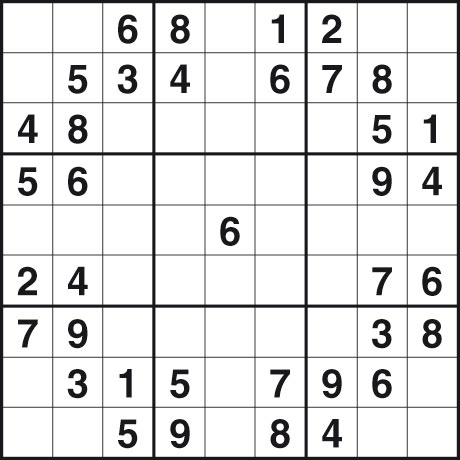
\includegraphics[width=5cm]{pics/sudoku}
\end{center}

\begin{exercise}
  Given the puzzle, what order should we handle unassigned variables? (line 3)
\end{exercise}

\censor{ Min-Remaining Values   Degree/ number of Factors heuristic}

\begin{exercise}
  Given the puzzle, what order should we assign values from $\mcD_i$? (line 4)
\end{exercise}
\censor{
   Least constraining value 
}

\section{Local Search}



Now we consider very different set of algorithms for solving CSPs. Up
into this point we have only looked at search algorithms that keep
track of incomplete assignments.  We saw in the last section that
standard search can be a poor fit for CSPs. For one, search inherently
requires a some of bookkeeping that can make it inefficient,
particularly with a large branching factor. More importantly when we
run DFS we may make a decision early on that makes it impossible to
satisfy the rest of the problem. This can lead the algorithm down very
costly dead-end paths when forward checking is not helpful.

In \textbf{local search}, instead of constructing a search tree using
consistent, partial assignments, we work in the inverse space of inconsistent,
complete assignments. We look for a consistent assignment by moving in
the local area of the current state.

\subsection{Complete Assignment Formalism}

The complete assignment formalism (complete state formalism in AIMA)  assumes that all non-goals states are inconsistent
complete assignments. Define the set $\mcS$ as giving all possible
complete assignments for a CSP.

Additionally for any complete assignment, we assume we have a function $\msc{Neighbors} : \mcS \rightarrow 2^{\mcS}$ that produces similar states. In the case of CSP this will give all complete assignments formed by changing the label of a single variable. For instance in graph coloring this might correspond to changing the color of one city, for tagging this might correspond to changing the tag of one word. 

% Note that when implementing we may want this function to be lazy, and not explicitly construct all neighboring assignments.

We also assume that we have a random function $\msc{Sample} : \mapsto \mcS$ that can give us a random initial assignment. When the domains are finite we can simply sample uniformly for each variable.  

% For the sake of these problems let assume that 
% we have the set of all goal states $\mcC  = \{s\in \mcS : \msc{Goal}(s) = 1\}$ and $f(s) $ 

% For certain problems this formulation makes sense. Consider 
% the case of translation. It is easy to reach. 

\vspace{1cm}
\begin{center}
\begin{tabularx}{\linewidth}{llX}
  \toprule
  Name & Value & Description \\
  \midrule
\\
 Neighbor & $\msc{Neighbors}: \mcS \mapsto 2^{\mcS}$ & \censor{Set of neighbors of each state.} \\\\
State Score & $f: \mcS \mapsto \reals$ & \censor{Score a state.} \\\\
Sample & $\msc{Sample} : \mapsto \mcS$ & \censor{Produce a random state.} \\ 
\bottomrule
\end{tabularx}
\end{center}

The neighbors and sample function can also in theory incorporate knowledge of the underlying domain. In practice this is often important. We might want to prune out obviously bad neighbors, or sample from distributions that are more likely to give partially consistent assignments.

For instance, in the homework we will return to the Sudoku
problem. For this problem our function $\msc{Sample}$ will sample from
assignments where all of the row factors are satisfied (but with
possibly inconsistent columns and boxes). The $\msc{Neighbors}$ function 
will consider all possible ways are flipping to elements of a row.
Since this operation keeps the rows consistent, local search spends 
much less time exploring inconsistent assignments. 


\vspace{1cm}
\ifthenelse{\isundefined{\StudentVersion}}{
\censor{}

}{
\censor{}
\vspace{5cm}
}



\subsection{Local Search Algorithms}

Local search refers to a large class of algorithms that work by
iteratively moving along the space of neighboring assignments. The underlying 
algorithm is remarkably simple:

\begin{algorithm}[h]
\begin{algorithmic}[1]
  \Procedure{LocalSearch}{}
  \State{$s \gets \msc{Sample}(\mcS)$}
  \For{$t = 1 \ldots \infty$}
  \State{s $\gets \msc{Local}(s, \msc{Neighbors}(s), t)$}
  \If{\censorm{$s$ is consistent}}
  \Return{$s$}
  \EndIf{}
  \EndFor{}
  \EndProcedure{}
\end{algorithmic}
\end{algorithm}

In this case \textsc{Local} is one of several possible local transition functions.  For each of these, we will use a cost or fitness function $f:\mcS \mapsto \reals$ 
which will estimate how far we are from a consistent assignment. For CSP 
there are two natural choices are:

\begin{enumerate}
\item Min Conflicts
  
  Count the number of remaining factors that are unsatisfied.
\item Weighted Conflicts
  
    Version of above where the factors are weighted.
\end{enumerate}

\subsection{Hill Climbing/Gradient Descent}

Let's begin with the simplest strategy. Here we will simply enumerate 
all neighbors and return the run that minimizes our cost function. 
This is known as the method of steepest descent.

\begin{algorithm}[h]
\begin{algorithmic}[1]
  \Procedure{SteepestDescent}{$s, \mcN, t$}
  \For{$s' \in \mcN$}
  \If{\censorm{$f(s') < f(s)$}}  $s \gets s'$
  \EndIf{}
  \EndFor{}
  \State{\Return{$s$}}
  \EndProcedure{}
\end{algorithmic}
\end{algorithm}

Alternatively we can return the value that first gives a descent direction, 
known as stochastic descent. This has the advantage of not requiring us
to enumerate the full set of neighbors.

\begin{algorithm}[h]
\begin{algorithmic}[1]
  \Procedure{StochasticDescent}{$s, \mcN, t$}
  \For{\censorm{$s' \in \mcN$ at random}}
  \If{\censorm{$f(s') < f(s)$}}  \Return{$ s'$}
  \EndIf{}
  \EndFor{}
  \State{\Return{$s$}}
  \EndProcedure{}
\end{algorithmic}
\end{algorithm}

However the problem with hill climbing/gradient descent methods is that they may quickly find a \textbf{local optima}, that is an assignment for which there are no neighbors with lower $f$. 

While the space of assignments is not continuous, this situation is analogous to finding a point with zero-gradient on a non-convex function, as shown in Figure~\ref{fig:siman}. When we are in this situation there is not local way to ``get out'' and find a different optimum. 

\subsection{Random Restarts}

One of the simplest way get out of this situation is with a random restart. If we alternate calls to gradient descent and random restart we move around the space hopefully exploring different local optima. 

\begin{algorithm}[h]
\begin{algorithmic}[1]
  \Procedure{RandomRestart}{$s, \mcN, t$}
  \If{\textsc{RestartSchedule}($t$)}  \Return{$\mathrm{Sample}(\mcS)$}
  \EndIf{}
  \State{\Return{$s$}}
  \EndProcedure{}
\end{algorithmic}
\end{algorithm}

One nice benefit of this algorithm is that we can run many random restarts in parallel since they never interact directly. However there are many functions of interest that can have a very large number of local minima, so even with this strategy we may not do much better.    

A similar approach is a method called local beam search or sometime Tabu search. This method keeps around the $K$-best assignments it has seen so far. At each step it checks the neighbors and recalculates the $K$-best list.   This algorithm can be combined with random restarts to refresh the list if all the assignments become too close.   

\begin{algorithm}[h]
\begin{algorithmic}[1]
  \Procedure{LocalBeamSearch}{}
  
  \For{$k = 1 \ldots K$ }
  \State{$s_k \gets \mathrm{Sample}(\mcS)$}
  \EndFor
  \For{$t = 1 \ldots \infty$ }
  \For{$k = 1 \ldots K$ }
  \For{$s' \in \msc{Neighbors}(s_k)$}
  \For{$k' = 1 \ldots K$ }
  \If{$f(s') < f(s_{k'})$} 
  \State{$s_j = s'$}
  \EndIf{}
  \EndFor{}
  \EndFor{}
  \EndFor{}
  \EndFor{}
  \EndProcedure{}
\end{algorithmic}
\end{algorithm}

This approach is similar to \textbf{genetic algorithms} another popular local search method described in AIMA.

\begin{figure}[h]
  \centering
  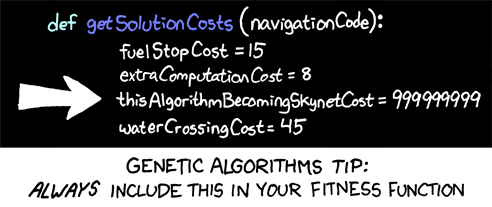
\includegraphics[width=10cm]{pics/genetic_algorithms}
  \caption{Subtext: Just make sure you don't have it maximize instead of minimize.}
\end{figure}

\subsection{Simulated Annealing}

Finally we consider a local algorithm that does not try to require making improvements at each step. This approach makes the assumption that early on we might want to bounce around a bit, but that later in the process we might fall back to gradient descent. 

To do the former, it randomly accepts some neighbors that increase $f$ based on how much worse they are. The likely of doing this decrease as we go, based on a predefined annealing schedule.

\begin{figure}
  \centering
  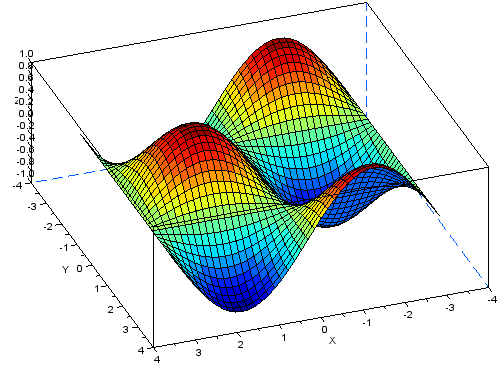
\includegraphics{pics/plot3d}
  \label{fig:siman}
  \caption{Graph with local minima and maxima.}
\end{figure}

\begin{algorithm}[h]
\begin{algorithmic}[1]
  \Procedure{SimulatedAnnealing}{$s, \mcN, t$}
  \State{$T \gets \msc{AnnealSchedule}(t)$}
  \State{$s' \gets \msc{Sample}(\mcN)$}
  \State{$\Delta E \gets f(s) - f(s')$}
  \State{$R \gets \mathrm{Rand}(0, 1)$}
  \If{$\Delta E > 0$ or $R > e^{\Delta E/ T}$}  \Return{$ s'$}
  \EndIf{}
  \State{\Return{$s$}}
  \EndProcedure{}
\end{algorithmic}

\end{algorithm}




\begin{figure}
  \centering
  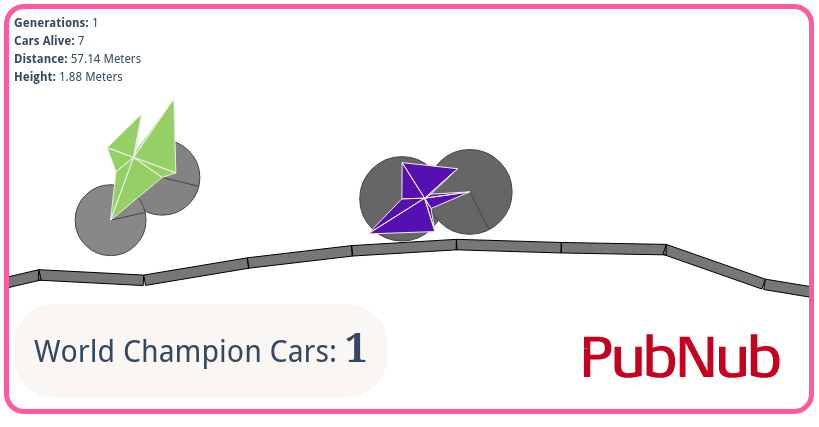
\includegraphics[width=\textwidth]{pics/genetic}
  \caption{Genetic algorithm car racing  (http://gencar.co/). Watch out, you can spend hours watching this. }
\end{figure}

 % \section{Integer Linear Programming}

\end{document}
